\documentclass{beamer}

% Should be documentclass beamer

\mode<presentation>
{
%  \usetheme[hideothersubsections]{PaloAlto}
  \usetheme{metropolis}
  \setbeamercovered{transparent}
}

\usepackage{amsfonts}
\usepackage{amsmath}
\usepackage{amssymb}
\usepackage{color}
\usepackage{tikz}
\usepackage{pgfplots}
\usepackage{listings}
\usepackage{courier}
%\usepackage[utf8]{inputenc}
%\usepackage[russian]{babel}

\lstset{
  numbers=left,
  basicstyle=\ttfamily\footnotesize,
  numberstyle=\tiny\color{gray},
  stepnumber=1,
  numbersep=10pt,
}

\newcommand{\iu}{\ensuremath{\mathrm{i}}}
\newcommand{\bbR}{\mathbb{R}}
\newcommand{\bbC}{\mathbb{C}}
\newcommand{\calV}{\mathcal{V}}
\newcommand{\calW}{\mathcal{W}}
\newcommand{\macheps}{\epsilon_{\mathrm{mach}}}
\newcommand{\matlab}{\textsc{Matlab}}

\newcommand{\ddiag}{\operatorname{diag}}
\newcommand{\fl}{\operatorname{fl}}
\newcommand{\nnz}{\operatorname{nnz}}
\newcommand{\tr}{\operatorname{tr}}
\renewcommand{\vec}{\operatorname{vec}}

\newcommand{\vertiii}[1]{{\left\vert\kern-0.25ex\left\vert\kern-0.25ex\left\vert #1
    \right\vert\kern-0.25ex\right\vert\kern-0.25ex\right\vert}}
\newcommand{\ip}[2]{\langle #1, #2 \rangle}
\newcommand{\ipx}[2]{\left\langle #1, #2 \right\rangle}
\newcommand{\order}[1]{O( #1 )}

\newcommand{\kron}{\otimes}


\newcommand{\hdr}[2]{
  \title[CS 5220, Fall 2017]{CS 5220: #2}
  \author{David Bindel}
  \date{#1}
}


\hdr{2017-09-21}{MPI Continued}

\begin{document}

\begin{frame}
  \titlepage
\end{frame}


\begin{frame}
  \frametitle{Logistics}

  \begin{itemize}
  \item HW 2 is up, due Mar 11 (overlap).
  \item HW 3 will go out start of next week.
  \end{itemize}
\end{frame}


\begin{frame}
  \frametitle{Previously on Parallel Programming}

  Can write a lot of MPI code with 6 operations we've seen:
  \begin{itemize}
  \item {\tt MPI\_Init}
  \item {\tt MPI\_Finalize}
  \item {\tt MPI\_Comm\_size}
  \item {\tt MPI\_Comm\_rank}
  \item {\tt MPI\_Send}
  \item {\tt MPI\_Recv}
  \end{itemize}
  ... but there are sometimes better ways.  Decide on
  communication style using simple performance models.

\end{frame}


\begin{frame}
  \frametitle{Communication performance}

  \begin{itemize}
  \item Basic info: {\em latency} and {\em bandwidth}
  \item Simplest model: $t_{\mathrm{comm}} = \alpha + \beta M$
  \item More realistic: distinguish CPU overhead from ``gap'' \\
    ($\sim$ inverse bw)
  \item Different networks have different parameters
  \item Can tell a lot via a simple ping-pong experiment
  \end{itemize}

\end{frame}


\begin{frame}
  \frametitle{Intel MPI on totient}

  \begin{itemize}
  \item Two six-core chips per nodes, eight nodes
  \item Heterogeneous network:
    \begin{itemize}
    \item Crossbar switch between cores (?)
    \item Bus between chips
    \item Gigabit ethernet between nodes
    \end{itemize}
  \item Default process layout (16 process example)
    \begin{itemize}
    \item Processes 0-5 on first chip, first node
    \item Processes 6-11 on second chip, first node
    \item Processes 12-17 on first chip, second node
    \item Processes 18-23 on second chip, second node
    \end{itemize}
  \item Test ping-pong from 0 to 1, 11, and 23.
  \end{itemize}

\end{frame}


\begin{frame}
  \frametitle{Approximate $\alpha$-$\beta$ parameters (on chip)}

  \begin{center}
    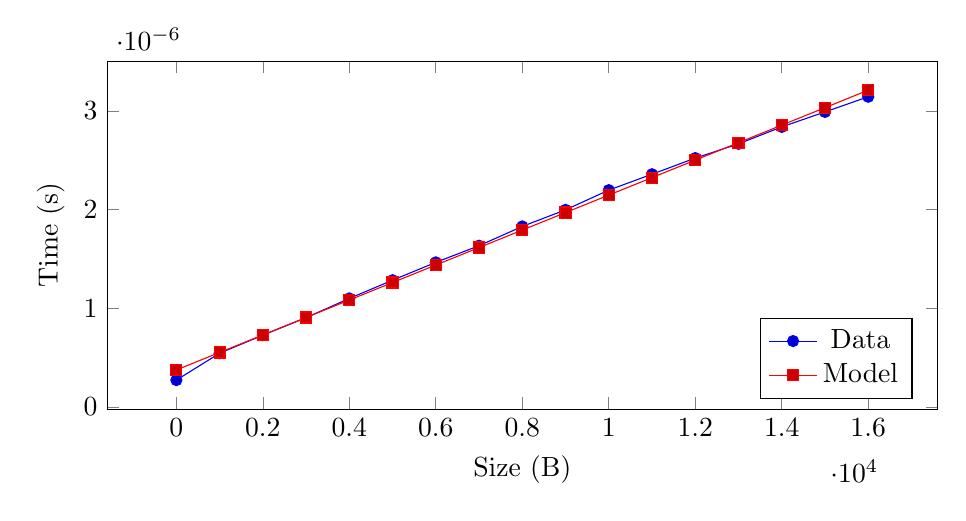
\begin{tikzpicture}
\begin{axis}[legend pos=south east,height=6cm,width=\textwidth,xlabel={Size (B)},ylabel={Time (s)}]
\addplot coordinates {
  (1,2.71035e-07)
  (1001,5.43535e-07)
  (2001,7.2711e-07)
  (3001,9.04125e-07)
  (4001,1.09977e-06)
  (5001,1.28422e-06)
  (6001,1.46538e-06)
  (7001,1.63429e-06)
  (8001,1.82995e-06)
  (9001,1.99816e-06)
  (10001,2.19826e-06)
  (11001,2.35945e-06)
  (12001,2.52297e-06)
  (13001,2.66729e-06)
  (14001,2.83954e-06)
  (15001,2.99131e-06)
  (16001,3.14512e-06)
};
\addlegendentry{Data}
\addplot coordinates {
  (1,3.74096e-07)
  (1001,5.51463e-07)
  (2001,7.2883e-07)
  (3001,9.06197e-07)
  (4001,1.08356e-06)
  (5001,1.26093e-06)
  (6001,1.4383e-06)
  (7001,1.61566e-06)
  (8001,1.79303e-06)
  (9001,1.9704e-06)
  (10001,2.14776e-06)
  (11001,2.32513e-06)
  (12001,2.5025e-06)
  (13001,2.67986e-06)
  (14001,2.85723e-06)
  (15001,3.0346e-06)
  (16001,3.21196e-06)
};
\addlegendentry{Model}
\end{axis}
\end{tikzpicture} \\
$\alpha \approx $ {\tt 3.74e-07},
$\beta \approx $ {\tt 1.77e-10}

  \end{center}
\end{frame}


\begin{frame}
  \frametitle{Approximate $\alpha$-$\beta$ parameters (cross-chip)}

  \begin{center}
    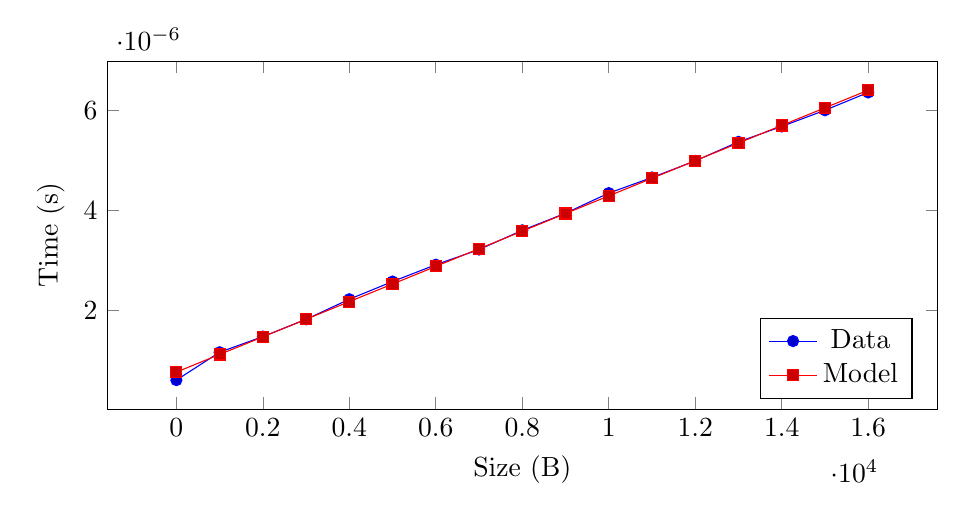
\begin{tikzpicture}
\begin{axis}[legend pos=south east,height=6cm,width=\textwidth,xlabel={Size (B)},ylabel={Time (s)}]
\addplot coordinates {
  (1,6.0302e-07)
  (1001,1.16096e-06)
  (2001,1.47426e-06)
  (3001,1.81971e-06)
  (4001,2.22256e-06)
  (5001,2.57663e-06)
  (6001,2.91378e-06)
  (7001,3.2172e-06)
  (8001,3.60213e-06)
  (9001,3.94472e-06)
  (10001,4.34748e-06)
  (11001,4.65996e-06)
  (12001,4.99168e-06)
  (13001,5.37362e-06)
  (14001,5.68144e-06)
  (15001,6.00605e-06)
  (16001,6.36241e-06)
};
\addlegendentry{Data}
\addplot coordinates {
  (1,7.63687e-07)
  (1001,1.11644e-06)
  (2001,1.4692e-06)
  (3001,1.82196e-06)
  (4001,2.17471e-06)
  (5001,2.52747e-06)
  (6001,2.88023e-06)
  (7001,3.23298e-06)
  (8001,3.58574e-06)
  (9001,3.9385e-06)
  (10001,4.29126e-06)
  (11001,4.64401e-06)
  (12001,4.99677e-06)
  (13001,5.34953e-06)
  (14001,5.70228e-06)
  (15001,6.05504e-06)
  (16001,6.4078e-06)
};
\addlegendentry{Model}
\end{axis}
\end{tikzpicture} \\
$\alpha \approx $ {\tt 7.63e-07},
$\beta \approx $ {\tt 3.53e-10}

  \end{center}
\end{frame}


\begin{frame}
  \frametitle{Approximate $\alpha$-$\beta$ parameters (cross-node)}

  \begin{center}
    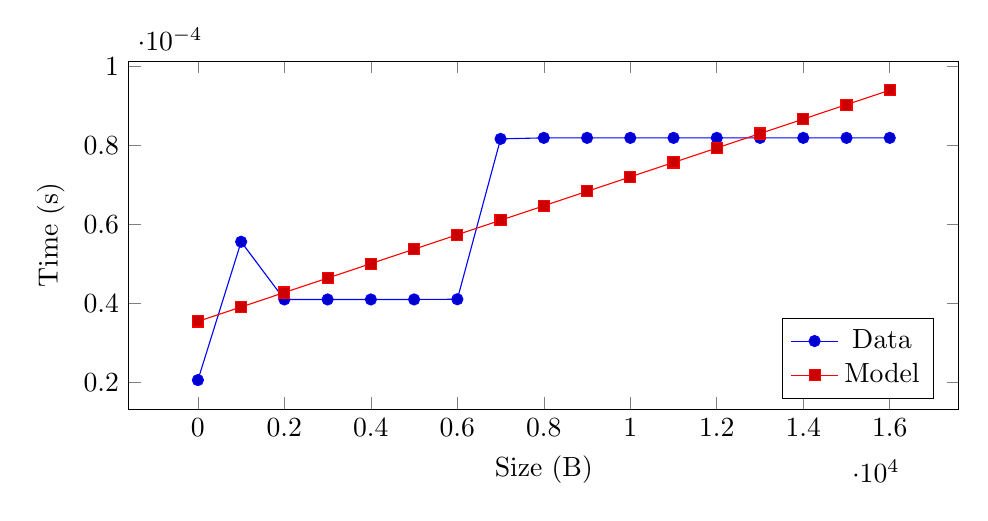
\begin{tikzpicture}
\begin{axis}[legend pos=south east,height=6cm,width=\textwidth,xlabel={Size (B)},ylabel={Time (s)}]
\addplot coordinates {
  (1,2.05185e-05)
  (1001,5.55847e-05)
  (2001,4.09613e-05)
  (3001,4.096e-05)
  (4001,4.09599e-05)
  (5001,4.0962e-05)
  (6001,4.10103e-05)
  (7001,8.16673e-05)
  (8001,8.19183e-05)
  (9001,8.19183e-05)
  (10001,8.19183e-05)
  (11001,8.19183e-05)
  (12001,8.19183e-05)
  (13001,8.19183e-05)
  (14001,8.19183e-05)
  (15001,8.19183e-05)
  (16001,8.19183e-05)
};
\addlegendentry{Data}
\addplot coordinates {
  (1,3.53888e-05)
  (1001,3.90526e-05)
  (2001,4.27164e-05)
  (3001,4.63803e-05)
  (4001,5.00441e-05)
  (5001,5.37079e-05)
  (6001,5.73717e-05)
  (7001,6.10355e-05)
  (8001,6.46993e-05)
  (9001,6.83632e-05)
  (10001,7.2027e-05)
  (11001,7.56908e-05)
  (12001,7.93546e-05)
  (13001,8.30184e-05)
  (14001,8.66822e-05)
  (15001,9.0346e-05)
  (16001,9.40099e-05)
};
\addlegendentry{Model}
\end{axis}
\end{tikzpicture} \\
$\alpha \approx $ {\tt 3.54e-05},
$\beta \approx $ {\tt 3.66e-09}

  \end{center}
\end{frame}


\begin{frame}
  \frametitle{Moral}

  Not all links are created equal!
  \begin{itemize}
  \item Might handle with mixed paradigm 
    \begin{itemize}
    \item OpenMP on node, MPI across
    \item Have to worry about thread-safety of MPI calls
    \end{itemize}
  \item Can handle purely within MPI
  \item Can ignore the issue completely?
  \end{itemize}
  For today, we'll take the last approach.

\end{frame}


\begin{frame}[fragile]
  \frametitle{Reminder: basic send and recv}

\begin{verbatim}
MPI_Send(buf, count, datatype, 
         dest, tag, comm);

MPI_Recv(buf, count, datatype,
         source, tag, comm, status);

\end{verbatim}

{\tt MPI\_Send} and {\tt MPI\_Recv} are {\em blocking}
\begin{itemize}
\item Send does not return until data is in system
\item Recv does not return until data is ready
\end{itemize}

\end{frame}


\begin{frame}
  \frametitle{Blocking and buffering}

  \begin{center}
    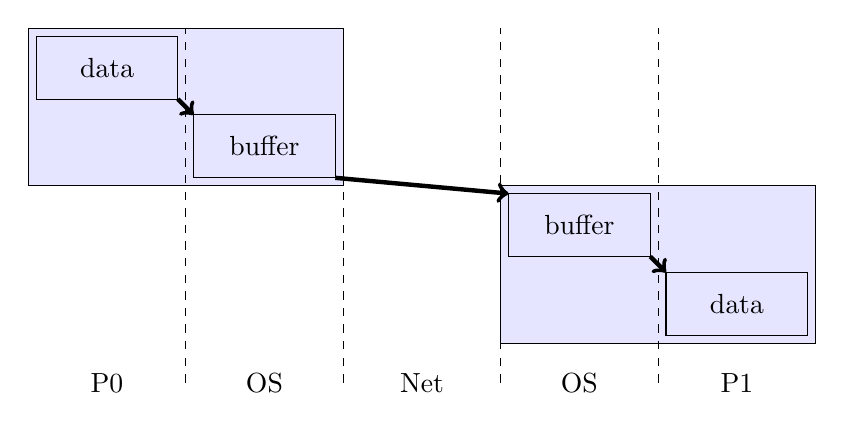
\begin{tikzpicture}
  \draw[fill=blue!10] (0,4) rectangle (4,2);
  \draw[fill=blue!10] (6,2) rectangle (10,0);
  \draw (0.1,3.9) rectangle (1.9,3.1);
  \draw (2.1,2.9) rectangle (3.9,2.1);
  \draw (6.1,1.9) rectangle (7.9,1.1);
  \draw (8.1,0.9) rectangle (9.9,0.1);
  \node at (1,3.5) {data};
  \node at (3,2.5) {buffer};
  \node at (7,1.5) {buffer};
  \node at (9,0.5) {data};
  \draw[dashed] (2,-0.5) -- (2,4);
  \draw[dashed] (4,-0.5) -- (4,4);
  \draw[dashed] (6,-0.5) -- (6,4);
  \draw[dashed] (8,-0.5) -- (8,4);
  \node at (1,-0.5) {P0};
  \node at (3,-0.5) {OS};
  \node at (5,-0.5) {Net};
  \node at (7,-0.5) {OS};
  \node at (9,-0.5) {P1};
  \draw [ultra thick,->] (1.9,3.1) -- (2.1,2.9);
  \draw [ultra thick,->] (7.9,1.1) -- (8.1,0.9);
  \draw [ultra thick,->] (3.9,2.1) -- (6.1,1.9);
\end{tikzpicture}

  \end{center}  
  Block until data ``in system'' --- maybe in a buffer?

\end{frame}


\begin{frame}
  \frametitle{Blocking and buffering}

  \begin{center}
    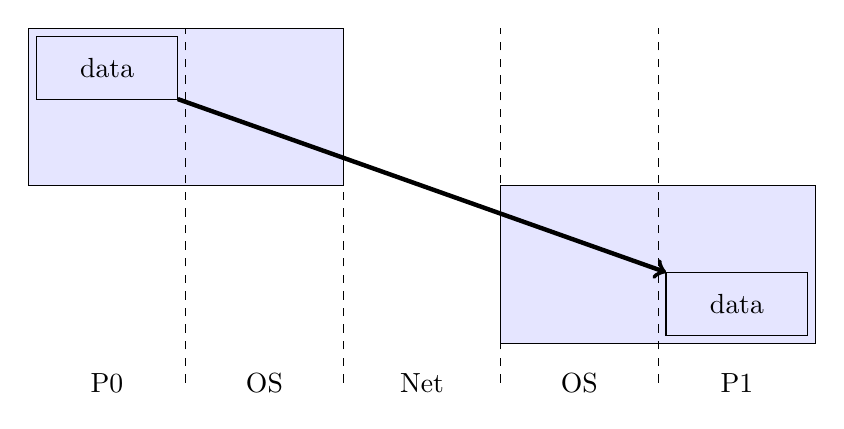
\begin{tikzpicture}
  \draw[fill=blue!10] (0,4) rectangle (4,2);
  \draw[fill=blue!10] (6,2) rectangle (10,0);
  \draw (0.1,3.9) rectangle (1.9,3.1);
  \draw (8.1,0.9) rectangle (9.9,0.1);
  \node at (1,3.5) {data};
  \node at (9,0.5) {data};
  \draw[dashed] (2,-0.5) -- (2,4);
  \draw[dashed] (4,-0.5) -- (4,4);
  \draw[dashed] (6,-0.5) -- (6,4);
  \draw[dashed] (8,-0.5) -- (8,4);
  \node at (1,-0.5) {P0};
  \node at (3,-0.5) {OS};
  \node at (5,-0.5) {Net};
  \node at (7,-0.5) {OS};
  \node at (9,-0.5) {P1};
  \draw [ultra thick,->] (1.9,3.1) -- (8.1,0.9);
\end{tikzpicture}

  \end{center}  
  Alternative: don't copy, block until done.

\end{frame}




\begin{frame}
  \frametitle{Problem 1: Potential deadlock}
  
  \begin{center}
    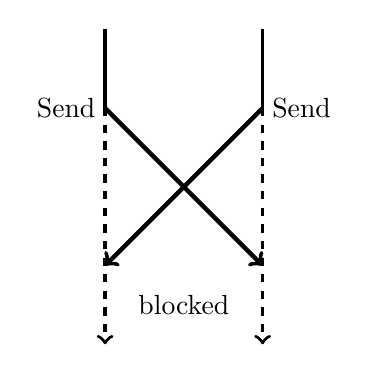
\begin{tikzpicture}
  \draw[very thick] (0,4) -- (0,3);
  \draw[very thick] (2,4) -- (2,3);
  \draw[very thick,dashed,->] (0,3) -- (0,0);
  \draw[very thick,dashed,->] (2,3) -- (2,0);
  \node[left]  at (0,3) {Send};
  \node[right] at (2,3) {Send};
  \node at (1,0.5) {blocked};
  \draw[ultra thick,->] (0,3) -- (2,1);
  \draw[ultra thick,->] (2,3) -- (0,1);
\end{tikzpicture}

  \end{center}
  Both processors wait to finish send before they can receive! \\
  May not happen if lots of buffering on both sides.

\end{frame}


\begin{frame}
  \frametitle{Solution 1: Alternating order}

  \begin{center}
    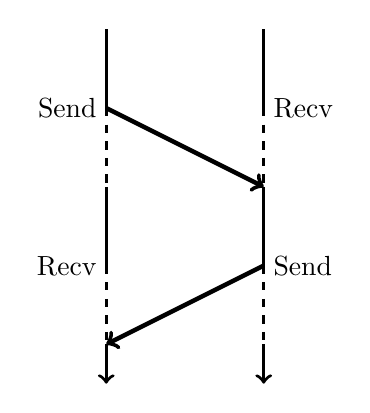
\begin{tikzpicture}
  \draw[very thick]        (0,4) -- (0,3);
  \draw[very thick,dashed] (0,3) -- (0,2);
  \draw[very thick]        (0,2) -- (0,1);
  \draw[very thick,dashed] (0,1) -- (0,0);
  \draw[very thick,->]     (0,0) -- (0,-0.5);
  \node[left] at (0,3) {Send};
  \node[left] at (0,1) {Recv};
  \draw[very thick]        (2,4) -- (2,3);
  \draw[very thick,dashed] (2,3) -- (2,2);
  \draw[very thick]        (2,2) -- (2,1);
  \draw[very thick,dashed] (2,1) -- (2,0);
  \draw[very thick,->]     (2,0) -- (2,-0.5);
  \node[right] at (2,3) {Recv};
  \node[right] at (2,1) {Send};
  \draw[ultra thick,->] (0,3) -- (2,2);
  \draw[ultra thick,->] (2,1) -- (0,0);
\end{tikzpicture}

  \end{center}
  Could alternate who sends and who receives.

\end{frame}


\begin{frame}
  \frametitle{Solution 2: Combined send/recv}

  \begin{center}
    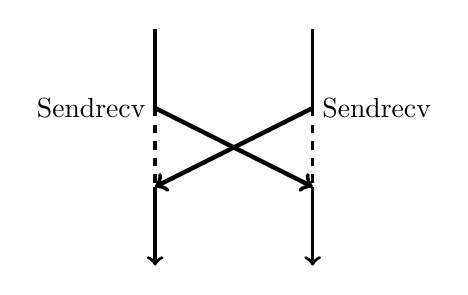
\begin{tikzpicture}
  \draw[very thick]        (0,3) -- (0,2);
  \draw[very thick,dashed] (0,2) -- (0,1);
  \draw[very thick,->]     (0,1) -- (0,0);
  \node[left] at (0,2) {Sendrecv};
  \draw[ultra thick,->]    (0,2) -- (2,1);
  \draw[very thick]        (2,3) -- (2,2);
  \draw[very thick,dashed] (2,2) -- (2,1);
  \draw[very thick,->]     (2,1) -- (2,0);
  \node[right] at (2,2) {Sendrecv};
  \draw[ultra thick,->]    (2,2) -- (0,1);
\end{tikzpicture}

  \end{center}
  Common operations deserve explicit support!

\end{frame}


\begin{frame}[fragile]
  \frametitle{Combined sendrecv}

\begin{verbatim}
MPI_Sendrecv(sendbuf, sendcount, sendtype,
             dest, sendtag, 
             recvbuf, recvcount, recvtype, 
             source, recvtag,
             comm, status);
\end{verbatim}
Blocking operation, combines send and recv to avoid deadlock.

\end{frame}


\begin{frame}
  \frametitle{Problem 2: Communication overhead}

  \begin{center}
    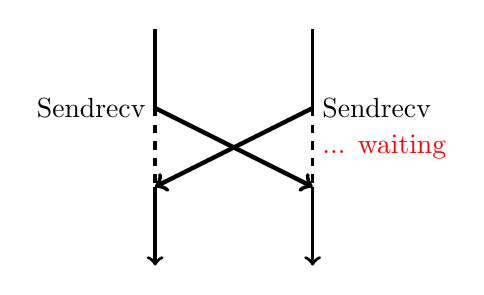
\begin{tikzpicture}
  \draw[very thick]        (0,3) -- (0,2);
  \draw[very thick,dashed] (0,2) -- (0,1);
  \draw[very thick,->]     (0,1) -- (0,0);
  \node[left] at (0,2) {Sendrecv};
  \draw[ultra thick,->]    (0,2) -- (2,1);
  \draw[very thick]        (2,3) -- (2,2);
  \draw[very thick,dashed] (2,2) -- (2,1);
  \draw[very thick,->]     (2,1) -- (2,0);
  \node[right] at (2,2) {Sendrecv};
  \draw[ultra thick,->]    (2,2) -- (0,1);
  \node[right] at (2,1.5) {\textcolor{red}{... waiting}};
\end{tikzpicture}

  \end{center}
  Partial solution: nonblocking communication
  
\end{frame}


\begin{frame}
  \frametitle{Blocking vs non-blocking communication}

  \begin{itemize}
  \item {\tt MPI\_Send} and {\tt MPI\_Recv} are {\em blocking}
    \begin{itemize}
    \item Send does not return until data is in system
    \item Recv does not return until data is ready
    \item Cons: possible deadlock, time wasted waiting
    \end{itemize}
  \item Why blocking?
    \begin{itemize}
    \item Overwrite buffer during send $\implies$ evil!
    \item Read buffer before data ready $\implies$ evil!
    \end{itemize}
  \item Alternative: {\em nonblocking} communication
    \begin{itemize}
    \item Split into distinct initiation/completion phases
    \item Initiate send/recv and promise not to touch buffer
    \item Check later for operation completion
    \end{itemize}
  \end{itemize}
\end{frame}


\begin{frame}
  \frametitle{Overlap communication and computation}

  \begin{center}
    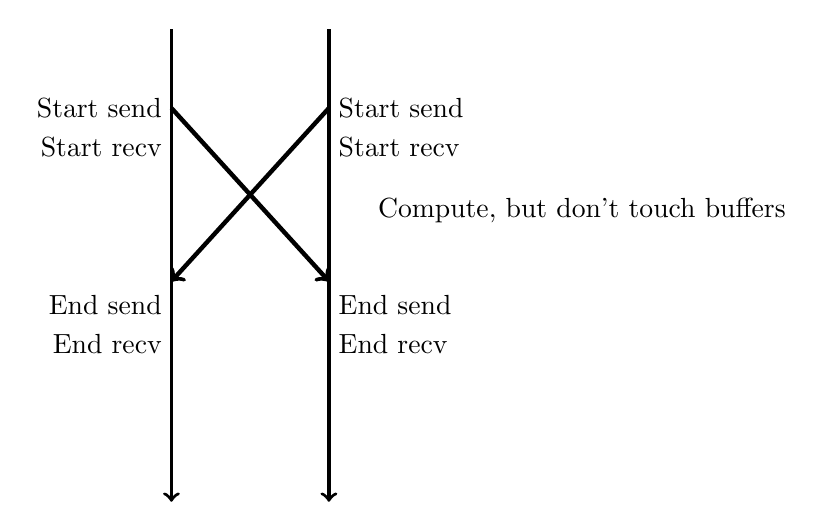
\begin{tikzpicture}
  \draw[very thick,->] (0,6) -- (0,0);
  \draw[very thick,->] (2,6) -- (2,0);
  \node[left]  at (0,5)   {Start send};
  \node[right] at (2,5)   {Start send};
  \node[left]  at (0,4.5) {Start recv};
  \node[right] at (2,4.5) {Start recv};
  \node[left]  at (0,2.5) {End send};
  \node[right] at (2,2.5) {End send};
  \node[left]  at (0,2)   {End recv};
  \node[right] at (2,2)   {End recv};
  \draw[ultra thick,->] (0,5) -- (2,2.8);
  \draw[ultra thick,->] (2,5) -- (0,2.8);
  \node[right] at (2.5,3.7) {Compute, but don't touch buffers};
\end{tikzpicture}

  \end{center}

\end{frame}


\begin{frame}[fragile]
  \frametitle{Nonblocking operations}

Initiate message:
\begin{verbatim}
MPI_Isend(start, count, datatype, dest
          tag, comm, request);
MPI_Irecv(start, count, datatype, dest
          tag, comm, request);
\end{verbatim}

\vspace{5mm}
Wait for message completion:
\begin{verbatim}
MPI_Wait(request, status);
\end{verbatim}

\vspace{5mm}
Test for message completion:
\begin{verbatim}
MPI_Test(request, status);
\end{verbatim}

\end{frame}


\begin{frame}[fragile]
  \frametitle{Multiple outstanding requests}

  Sometimes useful to have multiple outstanding messages:
\begin{verbatim}
MPI_Waitall(count, requests, statuses);
MPI_Waitany(count, requests, index, status);
MPI_Waitsome(count, requests, indices, statuses);
\end{verbatim}
  Multiple versions of test as well.

\end{frame}


\begin{frame}
  \frametitle{Other send/recv variants}

  Other variants of {\tt MPI\_Send}
  \begin{itemize}
  \item {\tt MPI\_Ssend} (synchronous) -- do not complete until
    receive has begun
  \item {\tt MPI\_Bsend} (buffered) -- user provides buffer 
    (via {\tt MPI\_Buffer\_attach})
  \item {\tt MPI\_Rsend} (ready) -- user guarantees receive has
    already been posted
  \item Can combine modes (e.g. {\tt MPI\_Issend})
  \end{itemize}
  {\tt MPI\_Recv} receives anything.

\end{frame}


\begin{frame}
  \frametitle{Another approach}

  \begin{itemize}
  \item Send/recv is one-to-one communication
  \item An alternative is one-to-many (and vice-versa):
    \begin{itemize}
    \item {\em Broadcast} to distribute data from one process
    \item {\em Reduce} to combine data from all processors
    \item Operations are called by all processes in communicator
    \end{itemize}
  \end{itemize}
\end{frame}


\begin{frame}[fragile]
  \frametitle{Broadcast and reduce}

\begin{verbatim}
MPI_Bcast(buffer, count, datatype,
          root, comm);
MPI_Reduce(sendbuf, recvbuf, count, datatype,
           op, root, comm);
\end{verbatim}

\begin{itemize}
\item {\tt buffer} is copied from root to others
\item {\tt recvbuf} receives result only at root
\item {\tt op} $\in \{$ {\tt MPI\_MAX}, {\tt MPI\_SUM}, \ldots $\}$
\end{itemize}
\end{frame}

\begin{frame}[fragile]
  \frametitle{Example: basic Monte Carlo}

\begin{verbatim}
#include <stdio.h>
#include <stdlib.h>
#include <mpi.h>
int main(int argc, char** argv) {
    int nproc, myid, ntrials = atoi(argv[1]);
    MPI_Init(&argc, &argv);
    MPI_Comm_size(MPI_COMM_WORLD, &nproc);
    MPI_Comm_rank(MPI_COMM_WORLD, &my_id);
    MPI_Bcast(&ntrials, 1, MPI_INT, 
              0, MPI_COMM_WORLD);
    run_trials(myid, nproc, ntrials);
    MPI_Finalize();
    return 0;
}
\end{verbatim}
\end{frame}


\begin{frame}[fragile]
  \frametitle{Example: basic Monte Carlo}

Let {\tt sum[0]} = $\sum_i X_i$ and {\tt sum[1]} = $\sum_i X_i^2$.
\begin{verbatim}
void run_mc(int myid, int nproc, int ntrials) {
    double sums[2] = {0,0};
    double my_sums[2] = {0,0};
    /* ... run ntrials local experiments ... */
    MPI_Reduce(my_sums, sums, 2, MPI_DOUBLE, 
               MPI_SUM, 0, MPI_COMM_WORLD);
    if (myid == 0) {
        int N = nproc*ntrials;
        double EX = sums[0]/N;
        double EX2 = sums[1]/N;
        printf("Mean: %g; err: %g\n", 
               EX, sqrt((EX*EX-EX2)/N));
    }
}
\end{verbatim}
\end{frame}


\begin{frame}
  \frametitle{Collective operations}

  \begin{itemize}
  \item Involve all processes in communicator
  \item Basic classes:
    \begin{itemize}
    \item Synchronization (e.g. barrier)
    \item Data movement (e.g. broadcast)
    \item Computation (e.g. reduce)
    \end{itemize}
  \end{itemize}
\end{frame}


\begin{frame}[fragile]
  \frametitle{Barrier}

\begin{verbatim}
MPI_Barrier(comm);
\end{verbatim}

Not much more to say.  Not needed that often.

\end{frame}


\begin{frame}
  \frametitle{Broadcast}

  \begin{center}
    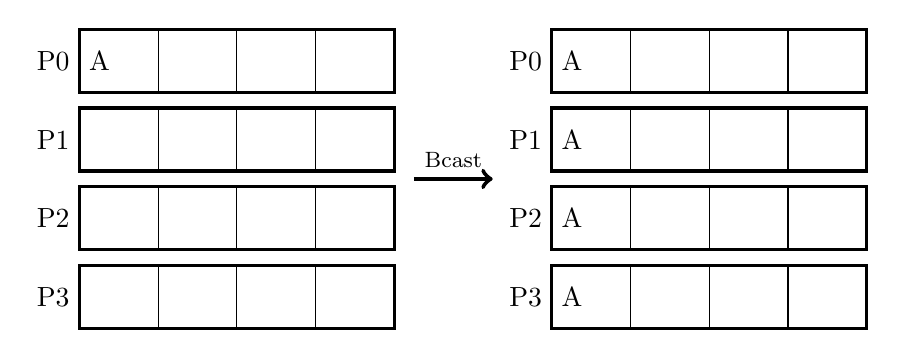
\begin{tikzpicture}
  \node[left] at (0,3.5) {P0};
\node[left] at (0,2.5) {P1};
\node[left] at (0,1.5) {P2};
\node[left] at (0,0.5) {P3};
\draw[very thick] (0,3.9) rectangle (4,3.1);
\draw[very thick] (0,2.9) rectangle (4,2.1);
\draw[very thick] (0,1.9) rectangle (4,1.1);
\draw[very thick] (0,0.9) rectangle (4,0.1);
\draw (1,3.1) -- (1,3.9);
\draw (1,2.1) -- (1,2.9);
\draw (1,1.1) -- (1,1.9);
\draw (1,0.1) -- (1,0.9);
\draw (2,3.1) -- (2,3.9);
\draw (2,2.1) -- (2,2.9);
\draw (2,1.1) -- (2,1.9);
\draw (2,0.1) -- (2,0.9);
\draw (3,3.1) -- (3,3.9);
\draw (3,2.1) -- (3,2.9);
\draw (3,1.1) -- (3,1.9);
\draw (3,0.1) -- (3,0.9);

  \draw[ultra thick,->] (4.25,2) -- (5.25,2)
       node[above,midway] {\footnotesize Bcast};
  \begin{scope}[xshift=6cm]
    \node[left] at (0,3.5) {P0};
\node[left] at (0,2.5) {P1};
\node[left] at (0,1.5) {P2};
\node[left] at (0,0.5) {P3};
\draw[very thick] (0,3.9) rectangle (4,3.1);
\draw[very thick] (0,2.9) rectangle (4,2.1);
\draw[very thick] (0,1.9) rectangle (4,1.1);
\draw[very thick] (0,0.9) rectangle (4,0.1);
\draw (1,3.1) -- (1,3.9);
\draw (1,2.1) -- (1,2.9);
\draw (1,1.1) -- (1,1.9);
\draw (1,0.1) -- (1,0.9);
\draw (2,3.1) -- (2,3.9);
\draw (2,2.1) -- (2,2.9);
\draw (2,1.1) -- (2,1.9);
\draw (2,0.1) -- (2,0.9);
\draw (3,3.1) -- (3,3.9);
\draw (3,2.1) -- (3,2.9);
\draw (3,1.1) -- (3,1.9);
\draw (3,0.1) -- (3,0.9);
      
  \end{scope}
  \node[right] at (0,3.5) {A};
  \node[right] at (6,3.5) {A};
  \node[right] at (6,2.5) {A};
  \node[right] at (6,1.5) {A};
  \node[right] at (6,0.5) {A};
\end{tikzpicture}

  \end{center}
\end{frame}


\begin{frame}
  \frametitle{Scatter/gather}

  \begin{center}
    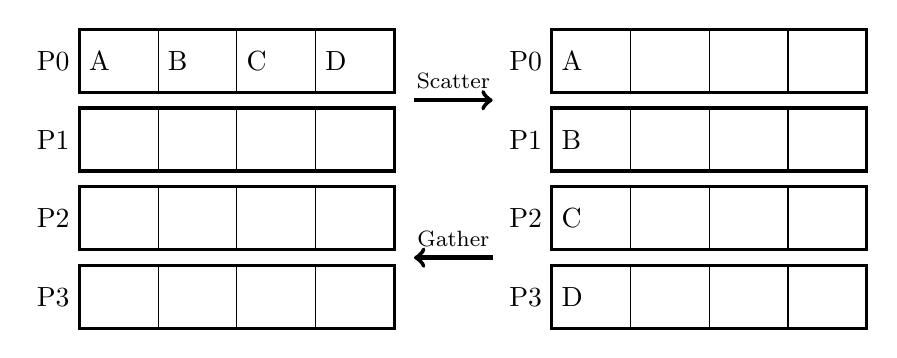
\begin{tikzpicture}
  \node[left] at (0,3.5) {P0};
\node[left] at (0,2.5) {P1};
\node[left] at (0,1.5) {P2};
\node[left] at (0,0.5) {P3};
\draw[very thick] (0,3.9) rectangle (4,3.1);
\draw[very thick] (0,2.9) rectangle (4,2.1);
\draw[very thick] (0,1.9) rectangle (4,1.1);
\draw[very thick] (0,0.9) rectangle (4,0.1);
\draw (1,3.1) -- (1,3.9);
\draw (1,2.1) -- (1,2.9);
\draw (1,1.1) -- (1,1.9);
\draw (1,0.1) -- (1,0.9);
\draw (2,3.1) -- (2,3.9);
\draw (2,2.1) -- (2,2.9);
\draw (2,1.1) -- (2,1.9);
\draw (2,0.1) -- (2,0.9);
\draw (3,3.1) -- (3,3.9);
\draw (3,2.1) -- (3,2.9);
\draw (3,1.1) -- (3,1.9);
\draw (3,0.1) -- (3,0.9);

  \draw[ultra thick,->] (4.25,3) -- (5.25,3)
       node[above,midway] {\footnotesize{Scatter}};
  \draw[ultra thick,->] (5.25,1) -- (4.25,1)
       node[above,midway] {\footnotesize{Gather}};
  \begin{scope}[xshift=6cm]
    \node[left] at (0,3.5) {P0};
\node[left] at (0,2.5) {P1};
\node[left] at (0,1.5) {P2};
\node[left] at (0,0.5) {P3};
\draw[very thick] (0,3.9) rectangle (4,3.1);
\draw[very thick] (0,2.9) rectangle (4,2.1);
\draw[very thick] (0,1.9) rectangle (4,1.1);
\draw[very thick] (0,0.9) rectangle (4,0.1);
\draw (1,3.1) -- (1,3.9);
\draw (1,2.1) -- (1,2.9);
\draw (1,1.1) -- (1,1.9);
\draw (1,0.1) -- (1,0.9);
\draw (2,3.1) -- (2,3.9);
\draw (2,2.1) -- (2,2.9);
\draw (2,1.1) -- (2,1.9);
\draw (2,0.1) -- (2,0.9);
\draw (3,3.1) -- (3,3.9);
\draw (3,2.1) -- (3,2.9);
\draw (3,1.1) -- (3,1.9);
\draw (3,0.1) -- (3,0.9);
      
  \end{scope}
  \node[right] at (0,3.5) {A};
  \node[right] at (1,3.5) {B};
  \node[right] at (2,3.5) {C};
  \node[right] at (3,3.5) {D};
  \node[right] at (6,3.5) {A};
  \node[right] at (6,2.5) {B};
  \node[right] at (6,1.5) {C};
  \node[right] at (6,0.5) {D};
\end{tikzpicture}

  \end{center}

\end{frame}


\begin{frame}
  \frametitle{Allgather}

  \begin{center}
    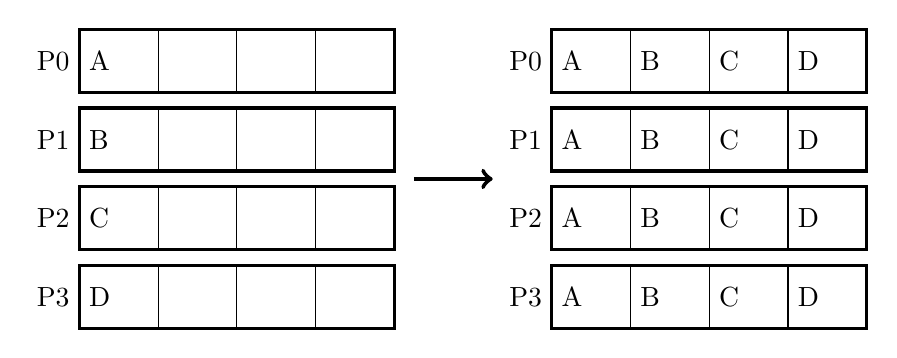
\begin{tikzpicture}
  \node[left] at (0,3.5) {P0};
\node[left] at (0,2.5) {P1};
\node[left] at (0,1.5) {P2};
\node[left] at (0,0.5) {P3};
\draw[very thick] (0,3.9) rectangle (4,3.1);
\draw[very thick] (0,2.9) rectangle (4,2.1);
\draw[very thick] (0,1.9) rectangle (4,1.1);
\draw[very thick] (0,0.9) rectangle (4,0.1);
\draw (1,3.1) -- (1,3.9);
\draw (1,2.1) -- (1,2.9);
\draw (1,1.1) -- (1,1.9);
\draw (1,0.1) -- (1,0.9);
\draw (2,3.1) -- (2,3.9);
\draw (2,2.1) -- (2,2.9);
\draw (2,1.1) -- (2,1.9);
\draw (2,0.1) -- (2,0.9);
\draw (3,3.1) -- (3,3.9);
\draw (3,2.1) -- (3,2.9);
\draw (3,1.1) -- (3,1.9);
\draw (3,0.1) -- (3,0.9);

  \draw[ultra thick,->] (4.25,2) -- (5.25,2);
  \begin{scope}[xshift=6cm]
    \node[left] at (0,3.5) {P0};
\node[left] at (0,2.5) {P1};
\node[left] at (0,1.5) {P2};
\node[left] at (0,0.5) {P3};
\draw[very thick] (0,3.9) rectangle (4,3.1);
\draw[very thick] (0,2.9) rectangle (4,2.1);
\draw[very thick] (0,1.9) rectangle (4,1.1);
\draw[very thick] (0,0.9) rectangle (4,0.1);
\draw (1,3.1) -- (1,3.9);
\draw (1,2.1) -- (1,2.9);
\draw (1,1.1) -- (1,1.9);
\draw (1,0.1) -- (1,0.9);
\draw (2,3.1) -- (2,3.9);
\draw (2,2.1) -- (2,2.9);
\draw (2,1.1) -- (2,1.9);
\draw (2,0.1) -- (2,0.9);
\draw (3,3.1) -- (3,3.9);
\draw (3,2.1) -- (3,2.9);
\draw (3,1.1) -- (3,1.9);
\draw (3,0.1) -- (3,0.9);
      
  \end{scope}
  \node[right] at (0,3.5) {A};
  \node[right] at (0,2.5) {B};
  \node[right] at (0,1.5) {C};
  \node[right] at (0,0.5) {D};
  \node[right] at (6,3.5) {A};
  \node[right] at (6,2.5) {A};
  \node[right] at (6,1.5) {A};
  \node[right] at (6,0.5) {A};
  \node[right] at (7,3.5) {B};
  \node[right] at (7,2.5) {B};
  \node[right] at (7,1.5) {B};
  \node[right] at (7,0.5) {B};
  \node[right] at (8,3.5) {C};
  \node[right] at (8,2.5) {C};
  \node[right] at (8,1.5) {C};
  \node[right] at (8,0.5) {C};
  \node[right] at (9,3.5) {D};
  \node[right] at (9,2.5) {D};
  \node[right] at (9,1.5) {D};
  \node[right] at (9,0.5) {D};
\end{tikzpicture}

  \end{center}

\end{frame}


\begin{frame}
  \frametitle{Alltoall}

  \begin{center}
    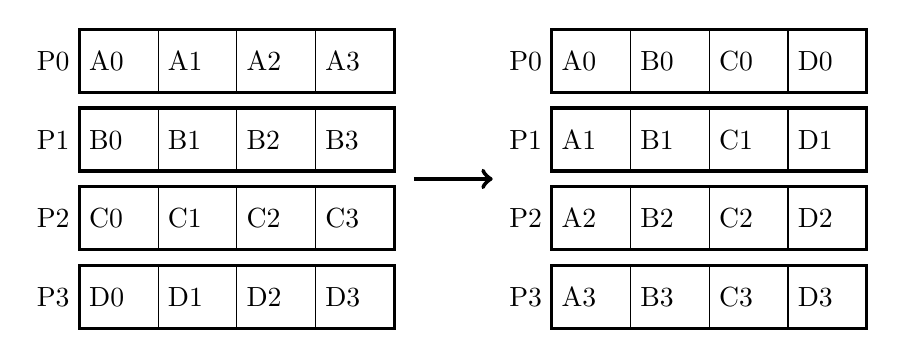
\begin{tikzpicture}
  \node[left] at (0,3.5) {P0};
\node[left] at (0,2.5) {P1};
\node[left] at (0,1.5) {P2};
\node[left] at (0,0.5) {P3};
\draw[very thick] (0,3.9) rectangle (4,3.1);
\draw[very thick] (0,2.9) rectangle (4,2.1);
\draw[very thick] (0,1.9) rectangle (4,1.1);
\draw[very thick] (0,0.9) rectangle (4,0.1);
\draw (1,3.1) -- (1,3.9);
\draw (1,2.1) -- (1,2.9);
\draw (1,1.1) -- (1,1.9);
\draw (1,0.1) -- (1,0.9);
\draw (2,3.1) -- (2,3.9);
\draw (2,2.1) -- (2,2.9);
\draw (2,1.1) -- (2,1.9);
\draw (2,0.1) -- (2,0.9);
\draw (3,3.1) -- (3,3.9);
\draw (3,2.1) -- (3,2.9);
\draw (3,1.1) -- (3,1.9);
\draw (3,0.1) -- (3,0.9);

  \draw[ultra thick,->] (4.25,2) -- (5.25,2);
  \begin{scope}[xshift=6cm]
    \node[left] at (0,3.5) {P0};
\node[left] at (0,2.5) {P1};
\node[left] at (0,1.5) {P2};
\node[left] at (0,0.5) {P3};
\draw[very thick] (0,3.9) rectangle (4,3.1);
\draw[very thick] (0,2.9) rectangle (4,2.1);
\draw[very thick] (0,1.9) rectangle (4,1.1);
\draw[very thick] (0,0.9) rectangle (4,0.1);
\draw (1,3.1) -- (1,3.9);
\draw (1,2.1) -- (1,2.9);
\draw (1,1.1) -- (1,1.9);
\draw (1,0.1) -- (1,0.9);
\draw (2,3.1) -- (2,3.9);
\draw (2,2.1) -- (2,2.9);
\draw (2,1.1) -- (2,1.9);
\draw (2,0.1) -- (2,0.9);
\draw (3,3.1) -- (3,3.9);
\draw (3,2.1) -- (3,2.9);
\draw (3,1.1) -- (3,1.9);
\draw (3,0.1) -- (3,0.9);
      
  \end{scope}
  \node[right] at (0,3.5) {A0};
  \node[right] at (1,3.5) {A1};
  \node[right] at (2,3.5) {A2};
  \node[right] at (3,3.5) {A3};
  \node[right] at (0,2.5) {B0};
  \node[right] at (1,2.5) {B1};
  \node[right] at (2,2.5) {B2};
  \node[right] at (3,2.5) {B3};
  \node[right] at (0,1.5) {C0};
  \node[right] at (1,1.5) {C1};
  \node[right] at (2,1.5) {C2};
  \node[right] at (3,1.5) {C3};
  \node[right] at (0,0.5) {D0};
  \node[right] at (1,0.5) {D1};
  \node[right] at (2,0.5) {D2};
  \node[right] at (3,0.5) {D3};
  \node[right] at (6,3.5) {A0};
  \node[right] at (6,2.5) {A1};
  \node[right] at (6,1.5) {A2};
  \node[right] at (6,0.5) {A3};
  \node[right] at (7,3.5) {B0};
  \node[right] at (7,2.5) {B1};
  \node[right] at (7,1.5) {B2};
  \node[right] at (7,0.5) {B3};
  \node[right] at (8,3.5) {C0};
  \node[right] at (8,2.5) {C1};
  \node[right] at (8,1.5) {C2};
  \node[right] at (8,0.5) {C3};
  \node[right] at (9,3.5) {D0};
  \node[right] at (9,2.5) {D1};
  \node[right] at (9,1.5) {D2};
  \node[right] at (9,0.5) {D3};
\end{tikzpicture}

  \end{center}

\end{frame}


\begin{frame}
  \frametitle{Reduce}

  \begin{center}
    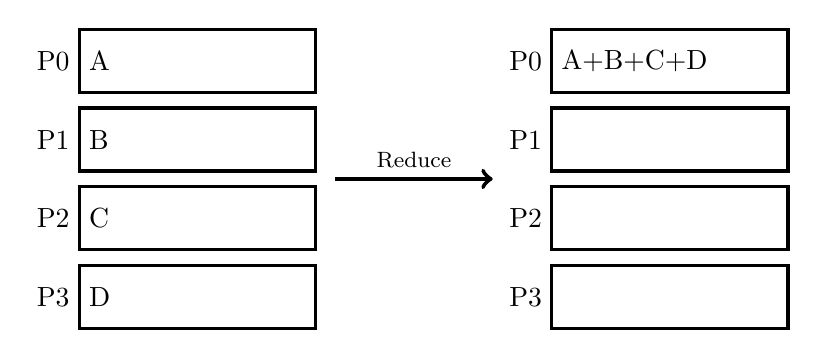
\begin{tikzpicture}
\node[left] at (0,3.5) {P0};
\node[left] at (0,2.5) {P1};
\node[left] at (0,1.5) {P2};
\node[left] at (0,0.5) {P3};
\draw[very thick] (0,3.9) rectangle (3,3.1);
\draw[very thick] (0,2.9) rectangle (3,2.1);
\draw[very thick] (0,1.9) rectangle (3,1.1);
\draw[very thick] (0,0.9) rectangle (3,0.1);

\draw[ultra thick,->] (3.25,2) -- (5.25,2)
     node[above,midway] {\footnotesize Reduce};
\begin{scope}[xshift=6cm]
  \node[left] at (0,3.5) {P0};
\node[left] at (0,2.5) {P1};
\node[left] at (0,1.5) {P2};
\node[left] at (0,0.5) {P3};
\draw[very thick] (0,3.9) rectangle (3,3.1);
\draw[very thick] (0,2.9) rectangle (3,2.1);
\draw[very thick] (0,1.9) rectangle (3,1.1);
\draw[very thick] (0,0.9) rectangle (3,0.1);

\end{scope}
\node[right] at (0,3.5) {A};
\node[right] at (0,2.5) {B};
\node[right] at (0,1.5) {C};
\node[right] at (0,0.5) {D};
\node[right] at (6,3.5) {A+B+C+D};
\end{tikzpicture}

  \end{center}

\end{frame}


\begin{frame}
  \frametitle{Scan}

  \begin{center}
    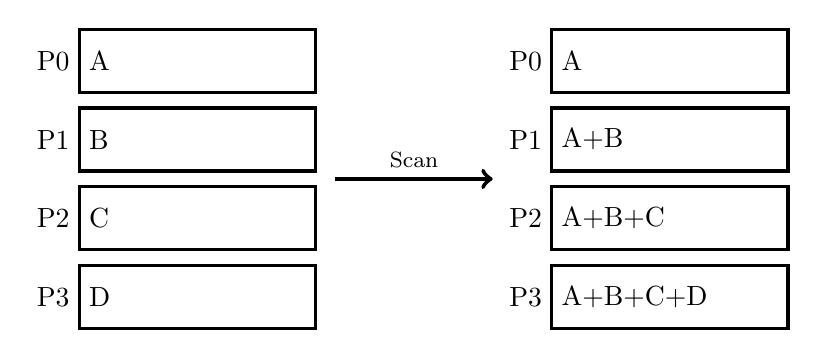
\begin{tikzpicture}
\node[left] at (0,3.5) {P0};
\node[left] at (0,2.5) {P1};
\node[left] at (0,1.5) {P2};
\node[left] at (0,0.5) {P3};
\draw[very thick] (0,3.9) rectangle (3,3.1);
\draw[very thick] (0,2.9) rectangle (3,2.1);
\draw[very thick] (0,1.9) rectangle (3,1.1);
\draw[very thick] (0,0.9) rectangle (3,0.1);

\draw[ultra thick,->] (3.25,2) -- (5.25,2)
     node[above,midway] {\footnotesize Scan};
\begin{scope}[xshift=6cm]
  \node[left] at (0,3.5) {P0};
\node[left] at (0,2.5) {P1};
\node[left] at (0,1.5) {P2};
\node[left] at (0,0.5) {P3};
\draw[very thick] (0,3.9) rectangle (3,3.1);
\draw[very thick] (0,2.9) rectangle (3,2.1);
\draw[very thick] (0,1.9) rectangle (3,1.1);
\draw[very thick] (0,0.9) rectangle (3,0.1);

\end{scope}
\node[right] at (0,3.5) {A};
\node[right] at (0,2.5) {B};
\node[right] at (0,1.5) {C};
\node[right] at (0,0.5) {D};
\node[right] at (6,3.5) {A      };
\node[right] at (6,2.5) {A+B    };
\node[right] at (6,1.5) {A+B+C  };
\node[right] at (6,0.5) {A+B+C+D};
\end{tikzpicture}

  \end{center}

\end{frame}


\begin{frame}
  \frametitle{The kitchen sink}

  \begin{itemize}
  \item In addition to above, have vector variants ({\tt v} suffix),
    more {\tt All} variants ({\tt Allreduce}), {\tt Reduce\_scatter}, ...
  \item MPI3 adds one-sided communication (put/get)
  \item MPI is {\em not} a small library!
  \item But a small number of calls goes a long way
    \begin{itemize}
    \item {\tt Init}/{\tt Finalize}
    \item {\tt Get\_comm\_rank}, {\tt Get\_comm\_size}
    \item {\tt Send}/{\tt Recv} variants and {\tt Wait}
    \item {\tt Allreduce}, {\tt Allgather}, {\tt Bcast}
    \end{itemize}
  \end{itemize}
\end{frame}


\end{document}
